\documentclass[10pt,nofootinbib,letterpaper]{revtex4}
%\usepackage[nocap]{ctex}

\usepackage{xeCJK}
% if \usrpackage{xetex} it will invoke the open source Fandol Song Font by default, which lack many Chinese characters
% Linux Requires TrueType Fonts from Windows (locating at C:\Windows\Fonts), and Simlink 
% ln -s blablabla /usr/share/fonts/WindowsFonts 
\setCJKmainfont[BoldFont={SimHei},ItalicFont={KaiTi}]{SimSun}
\setCJKfamilyfont{kaishu}{KaiTi} 
\newcommand*{\kaishu}{\CJKfamily{kaishu}}


\usepackage{amsmath,amssymb,amsfonts,mathrsfs,bm,dsfont}
\usepackage{slashed}
\usepackage{enumerate}
\usepackage{enumitem} % Customize itemize, see https://ctan.org/tex-archive/macros/latex/contrib/enumitem/
\usepackage[all]{xy}
\usepackage[noabbrev]{cleveref} % multiple equation ref, see https://tex.stackexchange.com/questions/314217/how-i-can-refer-multiple-equation-in-latex?rq=1
\usepackage[normalem]{ulem}	% delete line
\usepackage{array}
\usepackage{graphics,color}
\usepackage{tikz}
	\usetikzlibrary{calc}
	\usetikzlibrary{decorations.markings}
	\usetikzlibrary{arrows}
	\usetikzlibrary{patterns}
	%\usetikzlibrary{shapes.callouts}
\tikzset{
    level/.style = {
        ultra thick,
        blue,
    },
    connect/.style = {
        dashed,
        red
    },
    label/.style = {
        text width=2cm
    }
}
\usepackage{pgfplots}
%\usepackage[citestyle=authortitle]{biblatex} % able to cite the title, author and year
%\usepackage{hyperref}
\usepackage{feynmp} % feymann diagram
\usepackage{extarrows}
\usepackage[normalem]{ulem} % 文字划掉(横),与 cite 兼容问题,见 https://tex.stackexchange.com/questions/98222/ulem-incompatibility-with-multiple-entries-in-cite

\newcommand*\dd{\mathop{}\!\mathrm{d}}
\newcounter{Claim}[section]
\newenvironment{Claim}[1][]{{\par\normalfont\bfseries \underline{Claim~\stepcounter{Claim}\arabic{Claim}.}~#1~~}}{\par}
\newcounter{Property}[section]
\newenvironment{Property}[1][]{{\par\normalfont\bfseries \underline{Property~\stepcounter{Property}\arabic{Property}.}~#1~~}}{\par}
\newcounter{Proposition}[section]
\newenvironment{Proposition}[1][]{{\par\normalfont\bfseries \underline{Proposition~\stepcounter{Proposition}\arabic{Proposition}.}~#1~~}}{\par}
\newcounter{Theorem}[section]
\newenvironment{Theorem}[1][]{{\par\normalfont\bfseries \underline{Theorem~\stepcounter{Theorem}\arabic{Theorem}.}~#1~~}}{\par}
\newcounter{Note}[section]
\newenvironment{Note}[1][]{{\par\normalfont\bfseries \underline{Note~\stepcounter{Note}\arabic{Note}.}~#1~~}}{\par}
\newcounter{Lemma}[section]
\newenvironment{Lemma}[1][]{{\par\normalfont\bfseries \underline{Lemma~\stepcounter{Lemma}\arabic{Lemma}.}~#1~~}}{\par}
\newcounter{Corollary}[section]
\newenvironment{Corollary}[1][]{{\par\normalfont\bfseries \underline{Corollary~\stepcounter{Corollary}\arabic{Corollary}.}~#1~~}}{\par}
\newenvironment{Proof}{{\par~{\normalfont\bfseries $\vartriangleright$}~~}}{\hfill $\square$\par\hfill\par} %\par
\newcounter{Def}[section]
\newenvironment{Def}[1][]{{\par\normalfont\bfseries \underline{Definition~\stepcounter{Def}\arabic{Def}.}~#1~~}}{\par}
\newcounter{Assumption}[section]
\newenvironment{Assumption}[1][]{{\par\normalfont\bfseries \underline{Assumption~\stepcounter{Assumption}\arabic{Assumption}.}~#1~~}}{\par}



\allowdisplaybreaks[4] %允许 align 跨页编排

%\def\checkmark{\tikz\fill[scale=0.4](0,.35) -- (.25,0) -- (1,.7) -- (.25,.15) -- cycle;}
%\def\G{\mathcal{G}}
\def\Z{\mathcal{Z}}
\def\H{\mathcal{H}}
\def\D{\mathcal{D}}

\begin{document}
\title{Two Regimes of the Kitaev Materials: $\mathrm{Li}_2\mathrm{RhO}_3$ and $\mathrm{Ag}_3\mathrm{Li}\mathrm{Rh}_2\mathrm{O}_6$}
\author{Xiaodong Hu}

%\altaffiliation[Also at ]{Boson College}
\email{xiaodong.hu@bc.edu}
\affiliation{Department of Physics, Boston College}

\date{\today}

\begin{abstract}
	In this note, with the help of density-functional calculation and Hatree-Fock mean-field data, we build the low-energy effective Hamiltonians for two generation of Kitaev materials $\mathrm{Li}_2\mathrm{RhO}_3$ (LRO) and $\mathrm{Ag}_3\mathrm{Li}\mathrm{Rh}_2\mathrm{O}_6$ (ALRO). Particularly, we show that ALRO is controlled by the Kramers doublet, and the Ising-anisotropy exchange is the only possible one can write down. Furthermore, except for the common effects comming from spin-orbital coupling (SOC) and trigonal distortion, we notice that there is another geometric distortion that breaks the $\mathrm{RhO}_4$ coplane condition. Such distortion is neglegible for ALRO but commensurable in LRO.\par
	%\begin{center}
		\hfill\par
		{\centering\kaishu 尽挹西江,细斟北斗,万象为宾客。扣舷独啸,不知今夕何夕。\\[0.5em]}
	%\end{center}
	\hfill------ 张孝祥「水调歌头」
\end{abstract}

\maketitle
\tableofcontents

\section{Low-energy Effective Hamiltonian}
	A general strongly-interacting Hubbard-like Hamiltonian with rotational-invariant spin-spin interaction and arbitrary orbital degrees of freedom can be written as
	\begin{equation}\label{1.0.1}
		H=J_1\sum_{\langle ij \rangle}\bm{S}_i\cdot\bm{S}_j+\sum_{\langle ij \rangle}J_{2,ij}^{\alpha\beta}\tau_i^\alpha \tau_j^\beta+\sum_{\langle ij \rangle}J_{3,ij}^{\alpha\beta}(\bm{S}_j\cdot\bm{S}_j)(\tau_i^\alpha \tau_j^\beta)+\cdots.
	\end{equation}
	\indent Since there may be anisotropic terms for the orbital part of exchange like $\tau_i^z\tau_j^z,\tau_i^x\tau_j^x,\tau_i^x\tau_i^y$, etc., the general Hamiltonian \eqref{1.0.1} is really intractable for theoretical analysis. However, with the help of crystalline symmetry, in real materials many terms turn out to be vanishing. Particularly, we will show at the end of this section that, for ALRO, the allowed low-energy Hamiltonian can only be composed of Ising-like exchanges.

	\subsection{Octehedral Crystal Field}
		It is well-known in crystal field theory \cite{fazekas1999lecture} that the spherical symemtric $3d$-orbitals will split into two-fold $e_g$ orbitals (omitting the irrelevant radial part)
		\begin{equation*}
			|d_{x^2-y^2}\rangle=\dfrac{1}{\sqrt 2}(Y_2^{-2}+Y_2^2),\quad|d_{3z^2-r^2}\rangle=Y^0_2,
		\end{equation*}
		and three-fold $t_{2g}$ orbitals
		\begin{equation*}
			|d_{zx}\rangle=\dfrac{1}{\sqrt 2}(Y_2^{-1}-Y^1_2),\quad|d_{yz}\rangle=\dfrac{i}{\sqrt 2}(Y_2^{-1}+Y^1_2),\quad|d_{xy}\rangle=\dfrac{i}{\sqrt 2}(Y_2^{-2}-Y^2_2),
		\end{equation*}
		in the octahedral oxygen environment, with $Y_\ell^m(\theta,\phi)$ the familiar spherical harmonics, as is shown in FIG. \ref{fig:t2g-eg}.\par
		\begin{figure}[!htp]
			\centering
			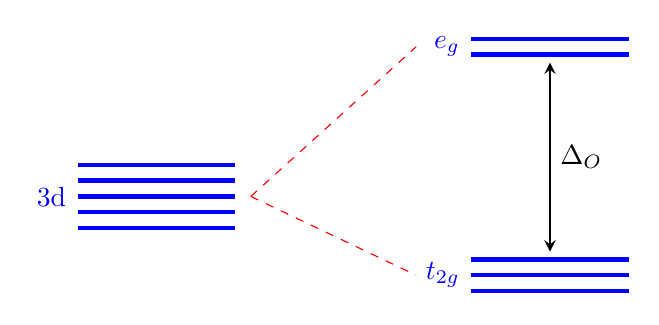
\begin{tikzpicture}
				% Draw all levels
				\draw[level] (0,0) -- (2,0);
				\draw[level] (0,-0.2) -- (2,-0.2);
				\draw[level] (0,-0.4) -- (2,-0.4);
				\draw[level] (0,0.2) -- (2,0.2);
				\draw[level] (0,0.4) -- (2,0.4);
				\draw[level] (0,0) node[left] {3d};

				\draw[connect] (2.2,0) -- (4.3,-1) (2.2,0) -- (4.3,1.9);
				
				\draw[level] (5,2) --  (7,2);
				\draw[level] (5,1.8) -- (7,1.8);
				\draw[level] (5,1.9) node[left] {$e_g$};

				\draw[level] (5,-0.8) -- (7,-0.8);
				\draw[level] (5,-1) -- (7,-1);
				\draw[level] (5,-1.2) -- (7,-1.2);
				\draw[level] (5,-1) node[left] {$t_{2g}$};

				\draw[<->,>=stealth,thick] (6,-0.7) -- node[right] {$\Delta_{O}$} (6,1.7);
				% Draw labels
				%\node[label] at (3.5,-3) {Octahedral Crystal Fields};
			\end{tikzpicture}
			\caption{\bf Octahedral Crystal Field Splitting.}
			\label{fig:t2g-eg}
		\end{figure}
		
		Depending on the energy scale between such $e_g$-$t_{2g}$ splitting $\Delta_O$ and spin-orbital coupling (SOC) $\Delta_{\text{SOC}}$, we will fall into high-spin and low-spin states with the electrons of $3d^5$ configuration on $\mathrm{Rh}^{3+}$. If $\Delta_{\text{SOC}}>\Delta_O$, by Hunds rule each orbital of $e_g$ and $t_{2g}$ will be half-filled to maximize the total spins, and we are in the high-spin state. In contrast, if the energy scale of $e_g$-$t_{2g}$ splitting is prominent (or at least comparable) $\Delta_O\geq\Delta_{\text{SOC}}$, then we are able to say that the five electrons occupy six degenerate (including spin degeneracy) $t_{2g}$ orbitals first, leaving only one empty hole so we are in the low-spin state.\par

		To determine which is the case, we can simply take a look at the numerical energy spectrum of relevant ten orbitals. The trick is to first turn off the SOC in the DFT calculation (It can be added back by hand in the analysis of our wannierized tight-binding model). The results are listed in TABLE. \ref{tab:LRO}.\par
		\begin{table}[!htp]
			\begin{tabular}{|c|c|c|}
				 & LRO without SOC & LRO with SOC\\
				\hline
						&8.72285690310658	& 8.67598932812092\\
	  					&8.72285690310658	& 8.675989328120933\\
				$t_{2g}$&8.752896854397369	& 8.730099641245802\\
						&8.752896854397376	& 8.730099641245813\\
						&8.819499295755385	& 8.884903534921547\\
						&8.819499295755387	& 8.88490353492155\\
						\hline
						&11.635763926129755	& 11.642613587390171\\
				$e_g$	&11.635763926129762	& 11.642613587390173\\
						&11.789525861249246	& 11.79621047265392\\
						&11.789525861249246	& 11.796210472653923
			\end{tabular}
			\hspace{2em}
			\begin{tabular}{|c|c|c|}
				 & ALRO without SOC & ALRO with SOC\\
				\hline
						&9.166541771379567	&9.142025045656869\\
	  					&9.166541771379569	&9.142025045656881\\
				$t_{2g}$&9.42234146297424	&9.371810987827514\\
						&9.422341462974245	&9.371810987827523\\
						&9.436907961253517	&9.50713680312438\\
						&9.436907961253526	&9.507136803124386\\
						\hline
						&12.329049772638278	&12.336116219990881\\
				$e_g$	&12.329049772638282	&12.336116219990888\\
						&12.406462151678134	&12.413564910334824\\
						&12.406462151678145	&12.41356491033483
			\end{tabular}
			\caption{Energy Spectrum of $3d$ Orbitals for both LRO and ALRO with/without SOC.}
			\label{tab:LRO}
		\end{table}
		Although the existence of SOC slightly shift both ten energy levels, the $e_g$-$t_{2g}$ splitting gap $\Delta_O^{\text{LRO}}\simeq2.94756\mathrm{eV}$ and $\Delta_O^{\text{ALRO}}\simeq3.0345\mathrm{eV}$ are large enough so that we can safely conclude that the discussion of low-energy physics can be confined in the subspace of $t_{2g}$ orbitals only. The name of orbitals can also be checked by their eigenstates and ???\par

		There is a well-known phenomena called \emph{$t_{2g}$-$p$ equivalence} \cite{sugano2012multiplets} stating that the \emph{effective} angular momentum within $t_{2g}$ subspace quench to have a similar form of that on $p$-orbitals
		\begin{equation}\label{1.1.1}
			\mathbf{L}|_{t_{2g}}=-\mathbf{L}|_{p}.
		\end{equation}
		This can be seen more clearly by rotating the aforementioned basis of $t_{2g}$-subspace to
		\begin{equation*}
			|+1\rangle\equiv\dfrac{1}{\sqrt 2}(|d_{zx}\rangle-i|d_{yz}\rangle)=Y_2^{-1},\quad |0\rangle\equiv i|d_{xy}\rangle=\dfrac{1}{\sqrt{2}}(Y_2^2-Y_2^{-2}),\quad|-1\rangle\equiv\dfrac{1}{\sqrt 2}(|d_{zx}\rangle-i|d_{yz}\rangle)=-Y_2^1.
		\end{equation*}
		and express the $5\times 5$ matrix of angular-momentum operator in the basis of $\{|+1\rangle,|0\rangle,|-1\rangle,|d_{3z^2-y^2}\rangle,|d_{x^2-y^2}\rangle\}$
		\begin{align*}
			L_x&=-\dfrac{1}{\sqrt 2}\left(\begin{array}{ccc|cc}
				0 & 1 & 0 & -\sqrt3 & -1\\
				1 & 0 & 1 & 0 & 0\\
				0 & 1 & 0 & \sqrt3 & 1\\
				\hline
				-\sqrt3 & 0 & \sqrt3 & 0 & 0\\
				-1 & 0 & 1 & 0 & 0
			\end{array}\right),\\[1em]
			L_y&=-\dfrac{i}{\sqrt{2}}\left(\begin{array}{ccc|cc}
				0 & 1 & 0 & \sqrt3 & 1\\
				-1 & 0 & 1 & 0 & 0\\
				0 & -1 & 0 & \sqrt3 & -1\\
				\hline
				-\sqrt3 & 0 & -\sqrt{3} & 0 & 0\\
				1 & 0 & 1 & 0 & 0
			\end{array}\right),\\[1em]
			L_z&=-\left(\begin{array}{ccc|cc}
				1 & 0 & 0 & 0 & 0\\
				0 & 0 & 0 & 0 & -2\\
				0 & 0 & -1 & 0 & 0\\
				\hline
				0 & 0 & 0 & 0 & 0\\
				0 & -2 & 0 & 0 & 0
			\end{array} \right).
		\end{align*}
		Clearly within the subspace of $t_{2g}$ ($3\times3$ block), the angular mometum operator takes exactly the form of that on the $\ell=1$ $p$-orbitals (off-diagonal compoents can be igonored due to the large gap $\Delta_O)$. While within the subspace of $e_g$ ($2\times2$ block), $\mathbf{L}|_{e_g}\equiv0$ and the further SOC are \emph{quenched}.\par
		But this is not the end of the story. Due to the competition between SOC and geometric distortion (here is trigonal distortion), we will end up with more fine structure of energy splitting on the $t_{2g}$ orbitals, as may be already noticed in TABLE \ref{tab:LRO}.
	
	\subsection{Spin-Orbital Coupling}
		When spin-orbital coupling (we denote $\bm{L}|_{t_{2g}}\equiv\bm{l}_{\text{eff}}$)
		\begin{equation}\label{1.2.1}
			H_{\text{SOC}}=\lambda\bm{l}_{\text{eff}}\cdot\bm{S}
		\end{equation}
		is dominant, which is the case for LRO, clearly the $t_{2g}$ triplet $l_{\text{eff}}=1$ and $S=1/2$ gives the $j=1/2$ doublet as the ground state, as is shown in FIG. \ref{fig:t2g-SOC}.
		\begin{figure}[!htp]
			\centering
			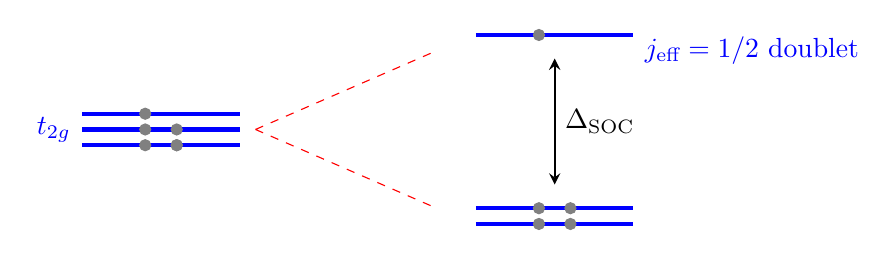
\begin{tikzpicture}
				% Draw all levels
				\draw[level] (0,0) -- (2,0);
				\draw[level] (0,0.2) -- (2,0.2);
				\draw[level] (0,-0.2) -- (2,-0.2);
				\draw[level] (0,0) node[left] {$t_{2g}$};
				\filldraw[gray] (0.8,0) circle (2pt);
				\filldraw[gray] (0.8,0.2) circle (2pt);
				\filldraw[gray] (0.8,-0.2) circle (2pt);
				\filldraw[gray] (1.2,0) circle (2pt);
				\filldraw[gray] (1.2,-0.2) circle (2pt);
				\filldraw[gray] (1.2,-0.2) circle (2pt);


				\draw[connect] (2.2,0) -- (4.5,-1) (2.2,0) -- (4.5,1);
				
				\draw[level] (5,1.2) --  (7,1.2);
				\draw[level] (7,1) node[right] {$j_{\text{eff}}=1/2$ doublet};
				\filldraw[gray] (5.8,1.2) circle (2pt);

				\draw[level] (5,-1) -- (7,-1);
				\draw[level] (5,-1.2) -- (7,-1.2);
				\filldraw[gray] (5.8,-1.2) circle (2pt);
				\filldraw[gray] (6.2,-1.2) circle (2pt);
				\filldraw[gray] (5.8,-1) circle (2pt);
				\filldraw[gray] (6.2,-1) circle (2pt);

				\draw[<->,>=stealth,thick] (6,-0.7) -- node[right] {$\Delta_{\text{SOC}}$} (6,0.9);
				% Draw labels
				%\node[label] at (3.5,-3) {Octahedral Crystal Fields};
			\end{tikzpicture}
			\caption{\bf Splitting from SOC.}
			\label{fig:t2g-SOC}
		\end{figure}
		The small splitting energy $\Delta_{\text{SOC}}\simeq0.0816\mathrm{eV}$ can be read from TABLE \ref{tab:LRO}.\par
		The superexchange can then be projected to such subspace through a $\tau=1/2$ pseoduspin operator. The effective Hamiltonian for strongly localized electrons ($U>J_H\gg t$) has already been well-studied for perovskites with $180^\circ$ exchange, e.g., $\mathrm{Sr}_2\mathrm{IrO}_4$, and $90^\circ$ exchange, i.e., $\mathrm{Na}_2\mathrm{IrO}_3$, in \cite{jackeli2009mott}. Since in LRO the $\mathrm{RhO}_6$ octahedra is edge-sharing, Jackeli and Khaliullin's result shows that the effective Hamiltonian is Kitaev-like \cite{kitaev2006anyons}
		\begin{equation}\label{1.2.2}
			H=-J\sum_{\langle ij \rangle }\mathcal{H}^{(\gamma)}_{ij}=-J\sum_{\langle ij \rangle}S_i^\gamma S_j^\gamma,
		\end{equation}
		where $\gamma=\{x,y,z\}$ labeling the types of $ij$-bonds.


	\subsection{Trigonal Distortion with SOC}
		In reality, chances are the $\mathrm{RhO}_6$ octahedra to be compressed or streched along $\hat{z}$ axis. Such trigonal crystal field breaks the $t_{2g}$ triplet into an $a_{1g}$ singlet \cite{landron2008importance}
		\begin{equation*}
			|a_{1g}\rangle\equiv|d_{3z^2-r^2}\rangle,
		\end{equation*}
		and $e_g'$ doublet
		\begin{equation*}
			|e'_{g1}\rangle\equiv\dfrac{2}{\sqrt 6}|d_{xy}\rangle-\dfrac{1}{\sqrt 3}|d_{zx}\rangle,\quad |e'_{g2}\rangle\equiv\dfrac{2}{\sqrt 6}|d_{x^2-y^2}\rangle-\dfrac{1}{\sqrt 3}|d_{yz}\rangle,
		\end{equation*}
		which is the case for our ALRO, as is show in FIG. \ref{fig:a1g-eg'}.
		\begin{figure}[!htp]
			\centering
			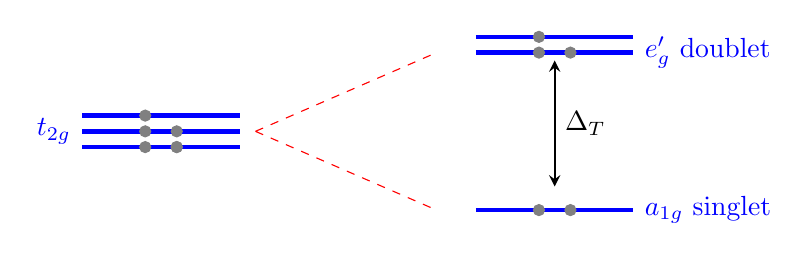
\begin{tikzpicture}
				% Draw all levels
				\draw[level] (0,0) -- (2,0);
				\draw[level] (0,0.2) -- (2,0.2);
				\draw[level] (0,-0.2) -- (2,-0.2);
				\draw[level] (0,0) node[left] {$t_{2g}$};
				\filldraw[gray] (0.8,0) circle (2pt);
				\filldraw[gray] (0.8,0.2) circle (2pt);
				\filldraw[gray] (0.8,-0.2) circle (2pt);
				\filldraw[gray] (1.2,0) circle (2pt);
				\filldraw[gray] (1.2,-0.2) circle (2pt);
				\filldraw[gray] (1.2,-0.2) circle (2pt);


				\draw[connect] (2.2,0) -- (4.5,-1) (2.2,0) -- (4.5,1);
				
				\draw[level] (5,1.2) --  (7,1.2);
				\draw[level] (5,1) -- (7,1);
				\draw[level] (7,1) node[right] {$e'_g$ doublet};
				\filldraw[gray] (5.8,1.2) circle (2pt);
				\filldraw[gray] (5.8,1) circle (2pt);
				\filldraw[gray] (6.2,1) circle (2pt);

				\draw[level] (5,-1) -- (7,-1);
				\draw[level] (7,-1) node[right] {$a_{1g}$ singlet};
				\filldraw[gray] (5.8,-1) circle (2pt);
				\filldraw[gray] (6.2,-1) circle (2pt);

				\draw[<->,>=stealth,thick] (6,-0.7) -- node[right] {$\Delta_{T}$} (6,0.9);
				% Draw labels
				%\node[label] at (3.5,-3) {Octahedral Crystal Fields};
			\end{tikzpicture}
			\caption{\bf Splitting from Trigonal Distortion.}
			\label{fig:a1g-eg'}
		\end{figure}
		This time the energy splitting is a little bit larger $\Delta_T=0.2630\mathrm{eV}$.\par
		Although a first glance of the four-fold degenerate $e'_g$ orbitals in FIG. \ref{fig:a1g-eg'} may pop up the idea that the effective orbital momentum to be $l_{\text{eff}}|_{e'_g}=3/2$, a careful representation of $\bm{l}_{\text{eff}}$ in the new basis of $\{|a_{1g}\rangle,|e'_{g1}\rangle,|e'_{g2}\rangle\}$ tells you NOT. In fact, the $t_{2g}$ effective orbital momentum operator now takes a strange form of
		\begin{equation}\label{1.3.1}
			l_{\text{eff},x}=\left(\begin{array}{c|cc}
				0 & \cdots &\\
				\hline
				\vdots & 0 & 0\\
				 & 0& 0
			\end{array}\right),\quad
			l_{\text{eff},y}=\left(\begin{array}{c|cc}
				0 & \cdots &\\
				\hline
				\vdots & 0 & 0\\
				 & 0& 0
			\end{array}\right),\quad
			l_{\text{eff},z}=\dfrac{1}{3}\left(\begin{array}{c|cc}
				0 & \cdots &\\
				\hline
				\vdots & 0 & -i\\
				 & i & 0
			\end{array}\right).
		\end{equation}
		Again due to the comparable large gap $\Delta_T$, we can safely narrow our discussion in the subspace of $e'_g$ orbitals, giving the only non-vanishing component of angular momentum matrix
		\begin{equation}\label{1.3.2}
			l_{\text{eff},z}|_{e'_g}\propto\left(\begin{array}{cc}
				0 &-i\\i & 0
			\end{array}\right)\equiv\tau^y.
		\end{equation}
		Therefore, the effective Hamiltonian \eqref{1.0.1} drastically simplify to
		\begin{equation}\label{1.3.3}
			H_{\text{eff}}=J_1\sum_{\langle ij \rangle}\bm{S}_i\cdot\bm{S}_j+\sum_{\langle ij \rangle}J_{2,ij}\tau_i^y\tau_i^y+\sum_{\langle ij \rangle }J_{3,ij}(\bm{S}_i\cdot\bm{S}_j)(\tau_i^y\tau_j^y)
		\end{equation}
		with Ising-anisotropy.\par
		The above discussion only consider the effect from trigonal distortion. Now if we take the SOC as a perturbation, by adding \eqref{1.3.3} with (all other components are suppressed in projection into the $e'_g$ subspace)
		\begin{equation}\label{1.3.4}
			H_{\text{SOC}}=\lambda\tau_yS_y,
		\end{equation}
		then clearly the low-energy state is of \emph{two-fold} degenerate
		\begin{equation}\label{1.3.5}
			|\mu_z=1\rangle\equiv|\tau_y=1,S_z=1/2\rangle,\quad |\mu_z=-1\rangle\equiv|\tau_y=-1,S_z=1/2\rangle,
		\end{equation}
		 forming a Kramers doublet.\par
		 Within the final low-energy subspace of $\{|\mu_z=\pm1\rangle\}$, the only possible exchange we can write down is of Ising-like
		 \begin{equation}\label{1.3.6}
		 	H_{\text{eff}}=\sum_{\langle ij \rangle}\mu_i^z\mu_j^z+\cdots.
		 \end{equation}
		 That is why we expect the ground state of ALRO to be in Ising-like phase (at least along one direction), and the $g$-factor will be anisotrpic.


	\subsection{Extra Distortion}
		As is shown in the numerical TABLE \ref{tab:LRO}, except for the above discussions of SOC and trigonal distortions, the fully-filled $j=3/2$ quadruplet of $t_{2g}$ orbitals are actually not perfectly degenerate. There exists an extra mecahnism splitting them, with a tiny gap about $\Delta_E^{\mathrm{LRO}}\simeq0.03\mathrm{eV}$, which is quite comparable with $\Delta_{\text{SOC}}$ (about $36.7\%$). A similar splitting occurs in ALRO, but the energy scale $\Delta_E^{\text{ALRO}}\simeq0.0146\mathrm{eV}$ is much smaller in comparison with $\Delta_T$ (about merely $5.56\%$).\par
		This can be ascribed to the extra distortion we find on the wannier centers of $\mathrm{RhO}_6$ octehedron: For the octahedron with merely trigonal distortion, the $\mathrm{RhO}_4$ plane should keep coplane. But a visualization of wannier centers evidently exihibit a violation of such coplane condition, as shown in FIG. \ref{fig:wannier}.\par
		\begin{figure}[!htp]
			\centering
			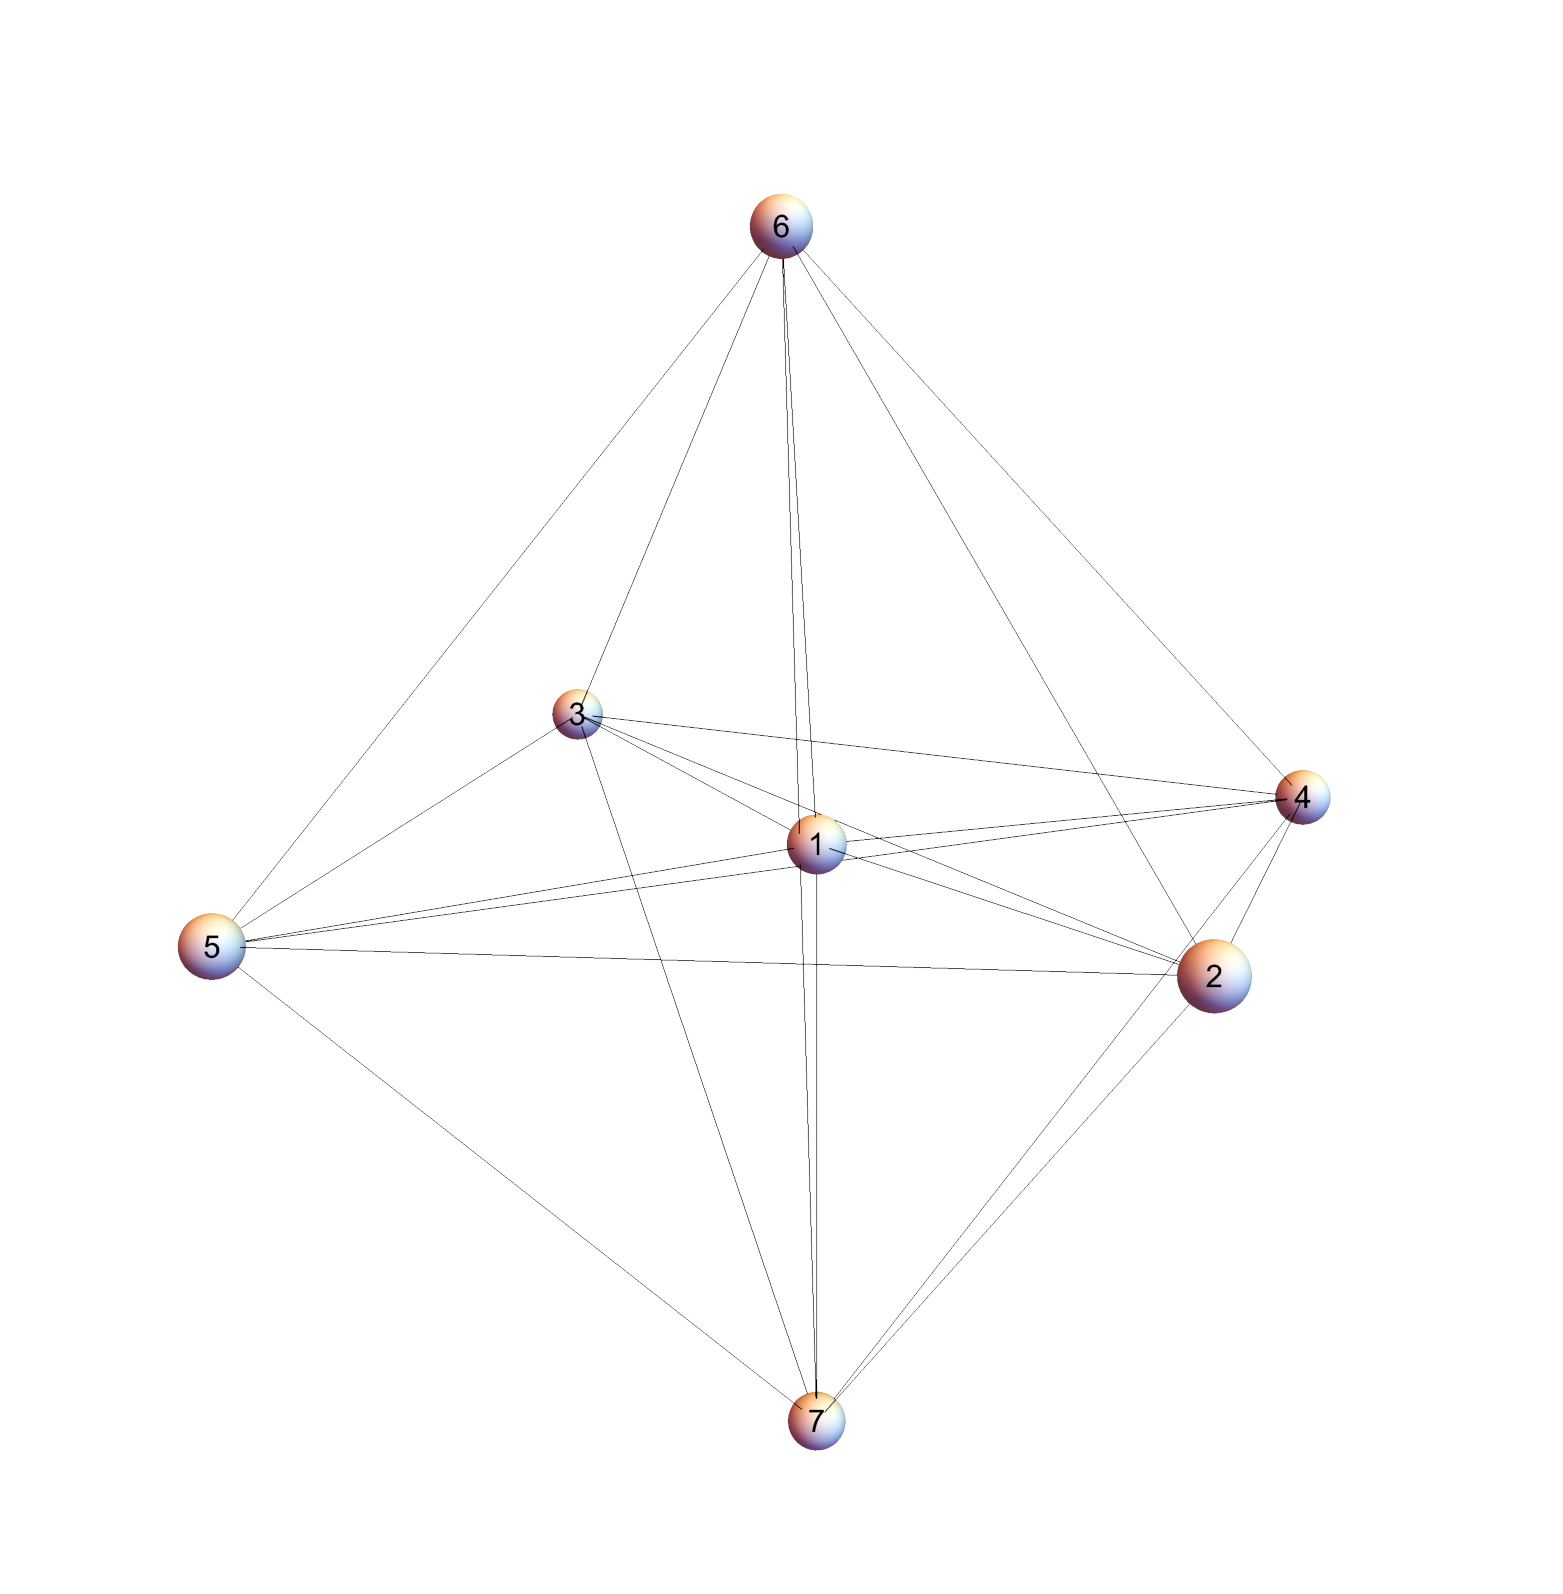
\includegraphics[scale=0.3]{LRO.pdf}
			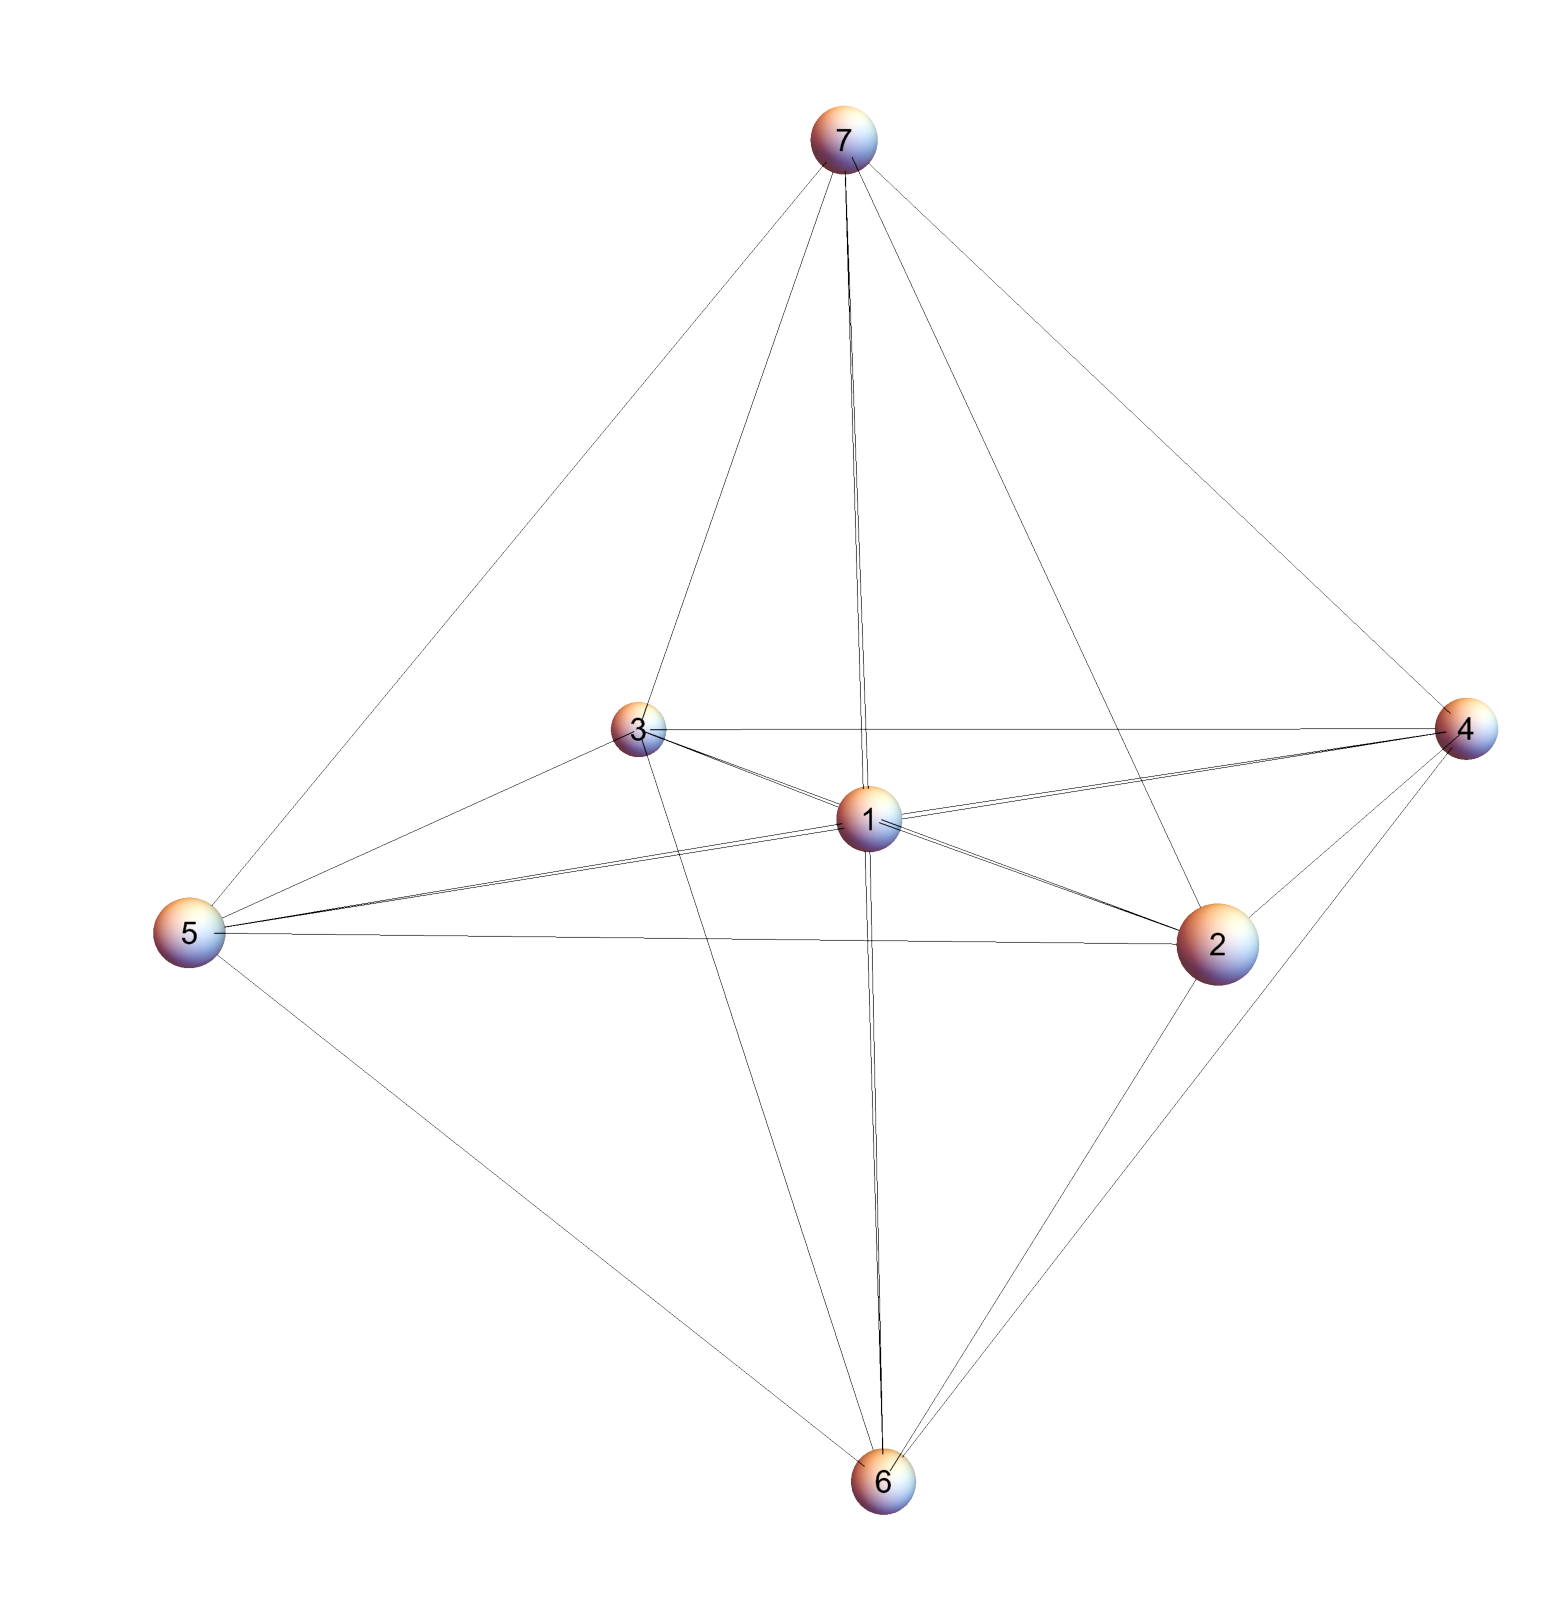
\includegraphics[scale=0.28]{ALRO.pdf}
			\caption{{\bf Wannier Centers of LRO and ALRO}: The left graphics is for LRO, while the right one is for ALRO. We draw the diagonal line to compare with the $\mathrm{O}$-$\mathrm{Rh}$-$\mathrm{O}$ plane. The discrepancy is in accordance with the strength of extra energy splitting we found in numerical results. Thus the extra distortion is much stronger in LRO than that for ALRO.}
			\label{fig:wannier}
		\end{figure}
		In light of this extra distortion, the Khaliullin's requirement of a \emph{strong} SOC may not be satisfied in LRO, and their effective Kitaev Hamiltonian may also not be accurate. While for ALRO we belive that the above low-energy analysis won't be altered.\par


\section{Long-Range Order}
	\subsection{LRO}
	\subsection{ALRO}

\bibliography{hxd}
\bibliographystyle{apsrev} % apsrev is format for PRL of APS
\end{document}